\documentclass[11pt]{article}
\usepackage{amssymb}
\usepackage{tipa}
\usepackage{amsmath}
\usepackage[scr]{rsfso}
\usepackage{graphicx}
\usepackage{float}

\newcommand{\then}{\rightarrow} 
\newcommand{\bicond}{\leftrightarrow}
\newcommand{\powerset}[1]{\mathscr{P}(#1)}
\newcommand{\family}[1]{\mathcal{#1}}

\title{\textbf{How to Prove It} \\ {\Large\itshape Daniel J. Velleman} \\ {\Large\itshape Chapter 3.5: Proofs Involving Disjunctions}}

\author{\textbf{Nathaniel Curnick} \\ \textit{Textbook Solutions}}

\date{}

%----------------------------------------------------------------------------------------

\begin{document}

\maketitle

\section*{Exercise 1}

Let $L = \{ \text{a, b, c, d, e} \}$ and $W = \{ \text{bad, bed, cab} \}$ .
Let $R = \{ (l, w) \in L \times W | \text{the letter } l \text{ occurs in the word } w \}$
Draw a diagram of $R$

\begin{figure}[H]
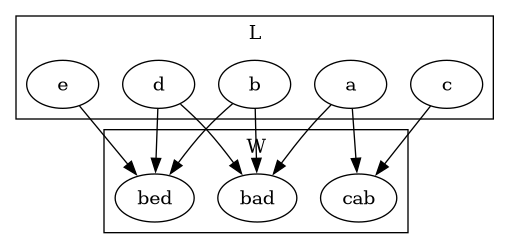
\includegraphics[width=0.5\textwidth]{4_3_images/4_3_1.png}
\end{figure}

\section*{Exercise 2}

Let $A = \{ \text{cat, dog, bird, rat} \}$ and let 
$R = \{(x, y) \in A \times A | \text{there is at least one letter that occurs in both of the words } x \text{ and } y \}$.
Draw a directed graph for the relation $R$. Is $R$ reflexive? Symmetric? Transitive?

\begin{figure}[H]
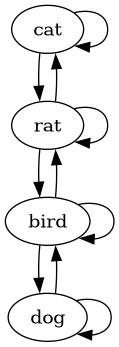
\includegraphics[height=0.25\textheight]{4_3_images/4_3_2.png}
\end{figure}

Reflexive and symmetric but not transitive.

\section*{Exercise 3}

Let $A = \{1, 2, 3, 4\}$. Draw a directed graph for $i_A$, the identity relation 
on $A$

\begin{figure}[H]
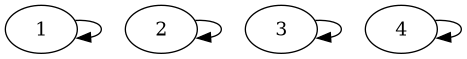
\includegraphics[width=0.5\textwidth]{4_3_images/4_3_3.png}
\end{figure}

\section*{Exercise 4}

List the ordered pairs in the relations represented by the directed graphs below.
Determine whether each relation is reflexive, symmetric or transitive

\begin{figure}[H]
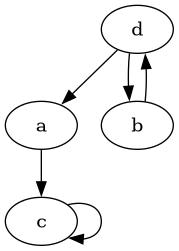
\includegraphics[height=0.25\textheight]{4_3_images/4_3_4a.png}
\end{figure}

$$\{ (a, b), (b, d), (c, c), (d, a), (d,b) \}$$

Not reflexive, symmetric or transitive

\begin{figure}[H]
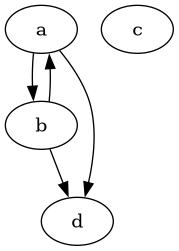
\includegraphics[height=0.25\textheight]{4_3_images/4_3_4b.png}
\end{figure}

$$\{ (a, b), (b,a), (b,d), (a,d)\}$$

Not reflexive, symmetric or transitive

\begin{figure}[H]
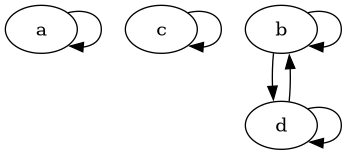
\includegraphics[height=0.25\textheight]{4_3_images/4_3_4c.png}
\end{figure}

$$\{(a,a), (c,c), (b,b), (b,d), (d,d), (d,b)\}$$

Reflexive, transitive and symmetric

\begin{figure}[H]
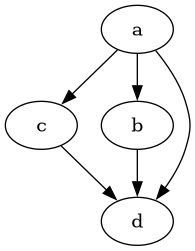
\includegraphics[height=0.25\textheight]{4_3_images/4_3_4d.png}
\end{figure}

$$\{(a,b), (a,c), (a,d), (b,d), (c,d)\}$$

Not reflexive or symmetric, but it is transitive

\section*{Exercise 5}

The following figure shows relations $R$ and $S$. Find $R \circ S$

\begin{figure}[H]
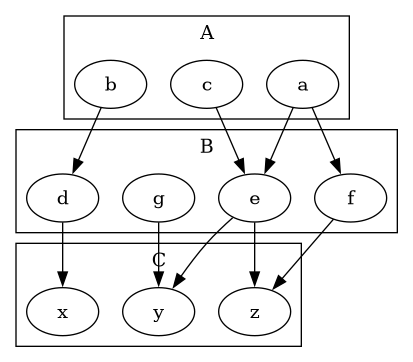
\includegraphics[width=0.5\textwidth]{4_3_images/4_3_5.png}
\end{figure}

$$S \circ R = \{ (a, y), (a, z), (b, x), (c, y), (c, z) \}$$

\section*{Exercise 6}

Suppose $r$ and $s$ are two positive real numbers. Let $D_r$ and $D_s$ be defined
as in part 3 of Example 4.3.1. What is $D_r \circ D_s$? 

$$D_r \circ D_s = D_{r+s}$$

Suppose $(x, y) \in D_r \circ D_s$. Then we choose some real number $z$ such that 
$(x, z) \in D_s$ and $(z, y) \in D_r$. This means that $| x - z | < s$ and
$| z - y | < r$. Therefore the inequality

$$|x-y| = |(x -z) + (z-y)| \leq |x-z| + |z-y| < r + s$$

So $(x, y) \in D_{r+s}$

Now, suppose $(x, y) \in D_{r+s}$, then $|x-y| < r+s$. Let $z = (rx + sy) / (r+s)$.
Then 

$$|x-z| = | x - \frac{rx + sy}{r+s} | = | \frac{sx - sy}{r+s} = 
\frac{s}{r+s} | x-y | < \frac{s}{r+s} (r+s) = s$$

So $(x,z) \in D_s$ and also

$$|z-y| = | \frac{rx + sy}{r+s} - y| = | \frac{rx - ry}{r+s}| = \frac{r}{r+s} |x-y| < \frac{r}{r+s} (r+s) = r$$

So $(z,y) \in D_r$. Therefore, $(x, y) \in D_r \circ D_s$.

\section*{Exercise 7}

Prove that $R$ is reflexive iff $i_A \subseteq R$, where $i_A$ is the identity relation on $A$

Suppose $R$ is reflexive. Let $(x, y)$ be an arbitrary element of $i_A$. Then, 
by definition of $i_A$, $x = y$. Since $R$ is reflexive then $(x, y) = (x, x) \in R$.
Since $(x, y)$ was arbitrary, this shows that $i_A \subseteq R$

Now suppose $i_A \subseteq R$. Let $x \in A$ be arbitrary. Then $(x, x) \in i_A$
so since $i_A \subseteq R$, then $(x, x) \in R$. Since $x$ was arbitrary, this 
shows $R$ is reflexive

\section*{Exercise 8}

Prove that $R$ is transitive iff $R \circ R \subseteq R$

Suppose $R$ is transitive. Let $(x, y)$ be an arbitrary element of $R \circ R$.
Then we can choose some arbitrary element $R \circ R$. Then we can choose some 
arbitrary element $z \in A$ such that $(x, z) \in R$ and $(z, y) \in R$. Since 
$R$ is transitive it follows that $(x, y) \in R$. Since $(x, y)$ was arbitrary
this shows that $R \circ R \subseteq R$

Suppose now that $R \circ R \subseteq R$. Suppose $(x, y) \in R$ and $(y, z) \in R$.
Then $(x, z) \in R \circ R$ and since $R \circ R \subseteq R$ it follows that 
$(x, z) \in R$. Since $x, y, z$ were arbitrary this shows that $R$ is transitive.

\section*{Exercise 9}

Suppose $A$ and $B$ are sets.

\noindent (a) Show that for every relation $R$ from $A$ to $B$, $R \circ i_A = R$

Suppose there is some $x \in A$ and $y \in B$. $i_A$ contains a relation from 
$x$ to $x$ by definition. Since $R$ contains relations from $A$ to $B$ and 
$i_A$ contains a relation from $A$ to $A$ then $R \circ i_A$ contains a relation
from $A$ to $B$. Since all elements in $i_A$ are from $x$ to $x$ then 
$R \circ i_A = R$.

\noindent (b) Show that for every relation $R$ from $A$ to $B$, $i_B \circ R = R$

Since $R$ contains a relation from $A$ to $B$ and $i_B$ contains a relation from 
$B$ to $B$ then $i_B \circ R$ contains a relation from $A$ to $B$. Suppse $y \in B$
then $i_B$ contains relations from $y$ to $y$. Thus, $i_B \circ R = R$

\section*{Exercise 10}

Suppose $S$ is a relation on $A$. Let $D = \text{Dom} (S)$ and $R = \text{Ran} (S)$.
Prove that $i_D \subseteq S^{-1} \circ S$ and $i_R \subseteq S \circ S^{-1}$

Let $D = \text{Dom} (S)$. $D$ contains all the inputs to $S$. $S^{-1} \circ S$ 
maps the input of $S$ to the output, then the output to the input. In other words,
it maps the input to the input. $i_D$ also maps the input to the input. Then 
$i_D \in S^{-1} \circ S$.

By symmetry $R$ is the output of $S$. $S \circ S^{-1}$ maps from the output to 
the output. Thus, $i_R \in S \circ S^{-1}$.

\section*{Exercise 11}

Suppose $R$ is a relation on $A$. Prove that if $R$ is reflexive then 
$R \subseteq R \circ R$

Suppose $R$ is a relation on $A$ and $R$ is reflexive. Suppose $(x, y) \in R$.
Since $R$ is reflexive, $(x, x) \in R$. Since $(x, x) \in R$ and 
$(x, y) \in R$ then $(x, y) \in R \circ R$. Thus, $R \subseteq R \circ R$.

\section*{Exercise 12}

Suppose $R$ is a relation on $A$

\noindent (a) Prove that if $R$ is reflexive, then so is $R^{-1}$.

$R$ is a relation on $A$. $R$ is reflexive, so by definition $i_A \subseteq R$.
Clearly, $i_A \subseteq R^{-1}$, thus $R^{-1}$ is also reflexive.

\noindent (b) Prove that if $R$ is symmetric, then so is $R^{-1}$

Suppose $R$ is symmetric. Let $x, y \in A$ be arbitrary and suppose 
$(x, y) \in R^{-1}$. Then $(y, x) \in R$. Since $R$ is symmetric then 
$(x, y) \in R$ so $(y, x) \in R^{-1}$. Thus, $R^{-1}$ is symmetric.

\noindent (c) Prove that if $R$ is transitive then so is $R^{-1}$.

Suppose $R$ is transitive. Suppose $x, y, z \in A$ and suppose $(x, y) \in R^{-1}$
and $(y, z) \in R^{-1}$. Then $(z, y) \in R$ and $(y, x) \in R$. Since $R$ is 
transitive, it follows that $(z, x) \in R$ so $(x, z) \in R^{-1}$. Thus, 
$R^{-1}$ is transitive.

\section*{Exercise 13}


Suppose $R_1$ and $R_2$ are relations on $A$. For each part, give either a 
proof or counterexample to justify your answer.

\noindent (a) If $R_1$ and $R_2$ are reflexive, must $R_1 \cup R_2$ be reflexive?

Yes. Since both $R_1$ and $R_2$ are reflexive, then 
$\forall x \in A ((x, x) \in R_1)$ and $\forall x \in A ((x, x) \in R_2)$.
So, $(x, x) \in R_1 \cup R_2$.

\noindent (b) If $R_1$ and $R_2$ are symetric, must $R_1 \cup R_2$ be symmetric?

Yes. Suppose $(x, y) \in R_1 \cup R_2$. Then, either $(x, y) \in R_1$ or 
$(x, y) \in R_2$. Since $(x, y) \in R_1$ and since $R_1$ is symmetric then 
$(y, x) \in R_1$ and thus $(y, x) \in R_1 \cup R_2$. By symmetry, the argument 
holds for $R_2$.

\noindent (c) If $R_1$ and $R_2$ are transitive, must $R_1 \cup R_2$ be transitive?

No. Consider $A = \{1, 2, 3\}$, $R_1 = \{(1, 2)\}, R_2 = \{(2, 3)\}$

\section*{Exercise 14}

Suppose $R_1$ and $R_2$ are relations on $A$. For each part, give either a 
proof or counterexample to justify your answer.

\noindent (a) If $R_1$ and $R_2$ are reflexive, must $R_1 \cap R_2$ be reflexive?

Yes. Suppose $(x, x) \in R_1$ and also $(x, x) \in R_2$. Since $(x, x)$ is in both
then $(x, x) \in R_1 \cap R_2$. Thus, $\forall x \in A ((x, x) \in R_1 \cap R_2)$,
which is the definition of reflexive


\noindent (b) If $R_1$ and $R_2$ are symetric, must $R_1 \cap R_2$ be symmetric?

Yes. Suppose $(x, y) \in R_1$ and $(x, y) \in R_2$. Since both are symmetric,
this means that $(x, y) \in R_1$ and $(y, x) \in R_2$. Since that is true then 
$(x, y) \in R_1 \cap R_2$ and $(y, x) \in R_1 \cap R_2$. Then $R_1 \cap R_2$
is symmetric

\noindent (c) If $R_1$ and $R_2$ are transitive, must $R_1 \cap R_2$ be transitive?

Yes. Suppose $(x, y) \in R_1 \cap R_2$ and $(y, z) \in R_1 \cap R_2$. Then 
$(x, y) \in R_1$ and $(y, z) \in R_1$ so since $R_1$ is transitive $(x, z) \in R_1$.
Similarly $(x, y) \in R_2$ and $(y, z) \in R_2$ so since $R_2$ is transitive
$(x, z) \in R_2$. Therefore, $(x, z) \in R_1 \cap R_2$.

\section*{Exercise 15}

Suppose $R_1$ and $R_2$ are relations on $A$. For each part, give either a 
proof or counterexample to justify your answer.

\noindent (a) If $R_1$ and $R_2$ are reflexive, must $R_1 \setminus R_2$ be reflexive?

No. If $(x, x) \in R_1$ and $(x, x) \in R_2$ (since $R_1$ and $R_2$ are reflexive)
then $(x, x) \notin R_1 \setminus R_2$. By definition, $R_1 \setminus R_2$ is not 
reflexive.

\noindent (b) If $R_1$ and $R_2$ are symetric, must $R_1 \setminus R_2$ be symmetric?

Yes. Suppose $R_1$ and $R_2$ are symmetric and suppose $(x, y) \in R_1 \setminus R_2$.
Then $(x, y) \in R_1$ and $(x, y) \notin R_2$. Since $(x, y) \in R_1$ and $R_1$ 
is symmetric then $(y, x) \in R_1$. Now suppose $(y, x) \in R_2$. Then since $R_2$
is symmetric, $(x, y) \in R_2$ which is a contradiction. Therefore, $(y, x) \notin R_2$.
Since $(y, x) \in R_1$ and $(y, x) \notin R_2$ then $(y, x) \in R_1 \setminus R_2$.

\noindent (c) If $R_1$ and $R_2$ are transitive, must $R_1 \setminus R_2$ be transitive?

No. Consider $A = \{1, 2, 3\}$, $R = \{(1, 2), (2, 3), (1, 3)\}$ and 
$R_2 = \{(1,3)\}$.

\section*{Exercise 16}

Suppose $R$ and $S$ are reflexive relations on $A$. Prove that $R \circ S$ is 
reflexive.

Since $R$ and $S$ are reflexive then $(x, x) \in R$ and $(x, x) \in S$. 
$R \circ S$ maps from the input to $S$ to the output of $S$ to the input of $R$ 
to the output of $R$. Since $(x, x) \in R$ and $(x, x) \in S$ we can map 
$(x, x) \in R \circ S$. Therefore, $R \circ S$ is reflexive.

\section*{Exercise 17}

Suppose $R$ and $S$ are symmetric relations on $A$. Prove that $R \circ S$ is 
symmetric iff $R \circ S = S \circ R$

Since $R$ and $S$ are symmetric then

$$R \circ S \text{ is symmetric iff } R \circ S = (R \circ S)^{-1}$$ 
$$R \circ S \text{ is symmetric iff } R \circ S = R^{-1} \circ S^{-1}$$ 
$$R \circ S \text{ is symmetric iff } R \circ S = S \circ R$$ 

\section*{Exercise 18}

Suppose $R$ ad $S$ are transitive relations on $A$. 
Prove that if $S \circ R \subseteq R \circ S$ then $R \circ S$ is transitive.

Suppose $S \circ R \subseteq R \circ S$. Suppose $(x, y) \in R \circ S$ and 
$(y, z) \in R \circ S$. Then, we can choose some $u, v \in A$ such that 
$(x, u) \in S$, $(u, y) \in R$. $(y, v) \in S$ and $(v, z) \in R$. 
Since $(u, y) \in R$ and $(y, v) \in S$ then $(u, v) \in S \circ R$. Since 
$S \circ R \subseteq R \circ S$ then $(u, v) \in R \circ S$. This means we can 
choose some $w \in A$ such that $(u, w) \in S$ and $(w, v) \in R$. Since 
$(x, u) \in S$ then $(u, w) \in S$ and $S$ is transitive so $(x, w) \in S$. 
Since $(w, v) \in R$ then $(v, z) \in R$ and $R$ is transitive so $(w, z) \in R$.
Since $(x, w) \in S$ and $(w, z) \in R$ then $(x, z) \in R \circ S$.

\section*{Exercise 19}

Consider the following putative theorem

\textbf{Theorem?} Suppose $R$ is a relation on $A$, and define relation $S$ on
$\powerset{A}$ as follows:

$$S = \{ (X, Y) \in \powerset{A} \times \powerset{A} | \exists x \in X \exists y \in Y  (x R y)\}$$

If $R$ is transitive, then so is $S$

\noindent (a) What's wrong with the following proof of the theorem?

\textit{Proof.} Suppose $R$ is transitive. Suppose $(X, Y) \in S$ and $(Y, Z) \in S$.
Then by the definition of $S$, $xRy$ and $yRz$, where $x \in X$, $y \in Y$ and 
$z \in Z$. Since $xRy$, $yRz$ and $R$ is transitive, $xRz$. But since $x \in X$
and $z \in Z$ it follows from the definition of $S$ that $(X, Y) \in S$. Thus,
$S$ is transitive

The issue is in the sentence ``then by the definition of $S$, $xRy$ and $yRz$ 
where $x \in X$, $y \in Y$ and $z \in Z$''. The problem is there is no reason 
for $y$ to be the same in $xRy$ and $yRz$. It would be more accurate to consider 
$xRy_1$ and $y_2 R z$.

\noindent (b) Is the theorem correct? Justify your answer with either a proof 
or a counterexample

No. Consider $A = \{1,2,3,4\}$, $B=\{(1,2), (3,4)\}$. Let $X = \{1\}$, $Y = \{2, 3\}$
and $Z = \{4\}$. Then $(X, Y) \in S$ and $(Y, Z) \in S$ but $(X, Z) \notin S$.

\section*{Exercise 20}

Suppose $R$ is a relation on $A$. Let $B = \{X \in \powerset{A} | X \neq \emptyset \}$
and define a relation $S$ as follows:

$$S = \{(X, Y) \in B \times B | \forall x \in X \forall y \in Y (xRy)\}$$

Prove that if $R$ is transitive, then so is $S$. Why did the empty set have to
be excluded from the set $B$ to make this proof work?

Suppose $R$ is transitive and suppose $(X, Y) \in S$ and $(Y, Z) \in S$. To prove 
that $(X, Z) \in S$ we would prove that $\forall x \in X \forall z \in Z (xRz)$.
Let $x \in X$ and $z \in Z$. Since $Y \in B, y \neq \emptyset$ so $y \in Y$.
Since $(X, Y) \in S$ and $(Y, Z) \in S$ by definition of $S$ we have $xRy$ and 
$yRz$. But since $R$ is transitive so $xRz$. We need to exclude the empty set so 
we can have $y \in Y$.

\section*{Exercise 21}

Suppose $R$ is a relation on $A$ and define a relation $S$ on $\powerset{A}$ as 
follows:

$$S = \{(X, Y) \in \powerset{A} \times \powerset{A} | \forall x \in X \exists y \in Y (xRy)\}$$

For each part, give either a proof or a counterexample to justify your answer

\noindent (a) if $R$ is reflexive, must $S$ be reflexive?

Yes. Let $X \in \powerset{A}$ be arbitrary. Let $x \in X$. Since $R$ is reflexive,
$xRx$. So, $\exists y \in X (xRy)$. Since $x$ was arbitrary, 
$\forall x \in X \exists y \in X (xRy)$, so $(X, X) \in S$.

\noindent (b) If $R$ is symmetric, must $S$ be symmetric?

No. Consider $A = \{1,2,3\}$, $R = \{(1,2), (2, 1)\}$ which is symmetric. 
Let $X = \{1\}$ and $Y = \{2, 3\}$. Then, $(X, Y) \in S$ but $(Y, X) \notin S$,
so $S$ is not symmetric

\noindent (c) If $R$ is transitive, must $S$ be transitive?

Yes. Suppose $R$ is transitive and $(X, Y) \in S$ and $(Y, Z) \in S$. Let $x \in X$
be arbitrary. Since $(X, Y) \in S$ we can choose some $y \in Y$ such that $xRy$.
Since $(Y, Z) \in S$ we can choose some $z \in Z$ such that $yRz$. By the fact 
$R$ is transitive since $xRy$ and $yRz$ then $xRz$. Since $x$ was arbitrary we 
conclude that $\forall x \in X \exists z \in Z (xRz)$, so $(X, Z) \in S$

\section*{Exercise 22}

Consider the following putative theorem

\textbf{Theorem?} Suppose $R$ is a relation on $A$. If $R$ is symmetric and 
transitive, then $R$ is reflexive.

Is the following proof correct? If so, what proof strategies does it use?
If not, can it be fixed? Is the theorem correct?

\textit{Proof?} Let $x$ be an arbitrary element of $A$. Let $y$ be any element
of $A$ such that $xRy$. Since $R$ is symmetric, it follows that $yRx$. But then
by transitivity, since $xRy$ and $yRx$ we can conclude that $xRx$. Since $x$ was 
arbitrary, we have shown that $\forall x \in A (xRx)$, so $R$ is reflexive

No, the mistake is in the sentence ``since $xRy$ and $yRx$ we can 
conclude that $xRx$''. You can't conclude this at all, consider 
$A = \{1\}, R = \emptyset$.

\section*{Exercise 23}

Suppose $A$ is a set, and $\family{F} \subseteq \powerset{A}$. Let
$R = \{(a,b) \in A \times A | \text{ for every } X \subseteq A \setminus \{a,b\}, 
\text{ if } X \cup \{a\} \in \family{F} \text{ then } X \cup \{b\} \in \family{F}\}$
Show that $R$ is transitive.

Suppose $aRb$ and $bRc$. To prove $aRc$ suppose $X \subseteq A \setminus \{a, c\}$
and $X \cup \{a\} \in \family{F}$. We must prove that $X \cup \{c\} \in \family{F}$.
If $c = a$ then $X \cup \{c\} = X \cup \{a\} \in \family{F}$. Now suppose if 
$c \neq a$. There are two cases

Case 1. $b \notin X$. Then $X \subseteq A \setminus \{a, b\}$. Since $aRb$
and $X \cup \{a\} \in \family{F}$ then $X \cup \{b\} \in \family{F}$.
But, also $bRc$ and $X \subseteq A \setminus \{b, c\}$ so since 
$X \cup \{b\} \in \family{F}$ then $X \cup \{c\} \in \family{F}$

Case 2. $b \in X$. Since $a \notin X$ and $c \notin X$, $b \neq a$ and 
$b \neq c$. Let $X_1 = X \cup \{a\} \setminus \{b\}$. Then 
$X_1 \subseteq A \setminus \{b, c\}$ and 
$X_1 \cup \{b\} = X \cup \{a\} \in \family{F}$. So, since $bRc$ then 
$X_1 \cup \{c\} \in \family{F}$. Note that 
$X_1 \cup \{c\} = X \cup \{a,c\} \setminus \{b\}$. Let 
$X_2 = X \cup \{c\} \setminus \{b\}$.
Then $X_2 \subseteq A \setminus \{a, b\}$ and 
$X_2 \cup \{a\} = X \cup \{a, c\} \setminus \{b\} = X_1 \cup \{c\} \in \family{F}$
so since $aRb$, $X_2 \cup \{b\} \in \family{F}$. But $X_2 \cup \{b\} = X \cup \{c\}$
so $X \cup \{c\} \in \family{F}$.

Therefore, $X \cup \{c\} \in \family{F}$. Since $X$ was arbitrary, this shows that 
$aRc$.

\section*{Exercise 24}

Let $R = \{(m,n) \in \mathbb{N} \times \mathbb{N} | |m - n| \leq 1\}$, which 
is a relation on $\mathbb{N}$

\noindent (a) Is $R$ reflexive on $\mathbb{N}$

Yes, because for every $n \in \mathbb{N}$, $|n - n| = 0 \leq 1$, so $(n,n) \in R$

\noindent (b) Is $R$ reflexive on $\mathbb{Z}$

No e.g. $(-1, -1) \notin R$


\end{document}
